\subsection{Grundbegriffe}

$G(V,E)$, $V$ = Vertices = Knoten, $E$ = Edges = Kanten

\begin{minipage}{0.5\textwidth}
\subsubsection*{Gerichteter Graph}
\begin{itemize}[leftmargin=*]
\item Kante geht nur in \textit{eine} Richtung
\end{itemize}\
\\
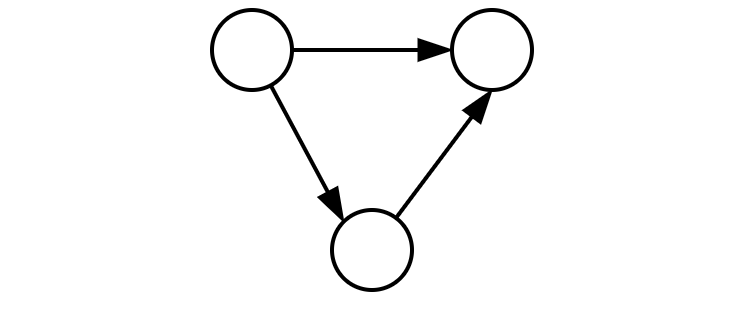
\includegraphics[width=0.6\textwidth]{graphics/graph_gerichtet.png}
\end{minipage}
\hfill
\begin{minipage}{0.5\textwidth}
\subsubsection*{Ungerichteter Graph}
\begin{itemize}[leftmargin=*]
\item Kante geht nur in \textit{beide} Richtung
\end{itemize}\
\\
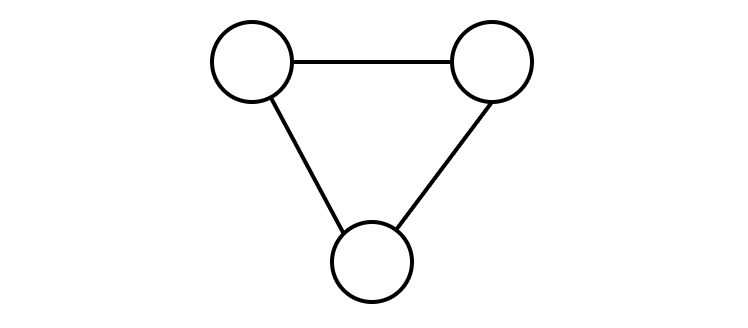
\includegraphics[width=0.6\textwidth]{graphics/graph_ungerichtet.png}
\end{minipage}


\begin{minipage}{0.5\textwidth}
\subsubsection*{Zusammenhängender Graph}
\begin{itemize}[leftmargin=*]
\item Verbindung von einem Knotenpunkt zu allen anderen
\item Verbindungen müssen nicht direkt sein
\item Gibt keine isolierten Knoten
\end{itemize}\
\\
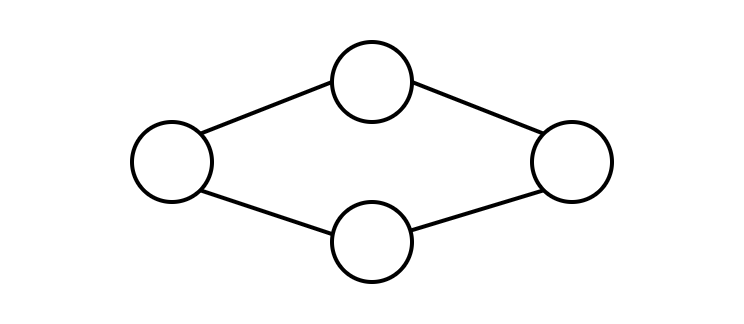
\includegraphics[width=0.6\textwidth]{graphics/graph_zusammen.png}
\end{minipage}
\hfill
\begin{minipage}{0.5\textwidth}
\subsubsection*{Nichtzusammenhängender Graph}
\begin{itemize}[leftmargin=*]
\item Wenn ein Knoten isoliert ist und keine Verbindung herrscht
\end{itemize}\
\\
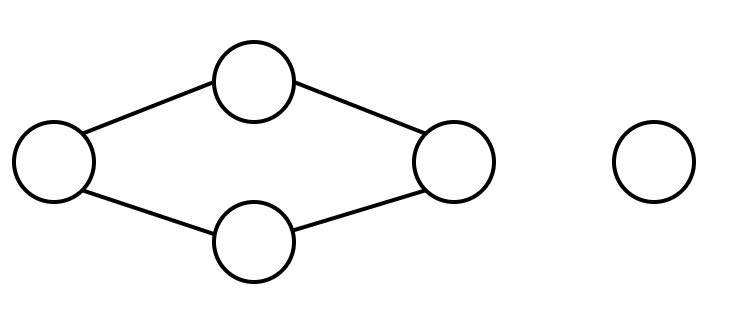
\includegraphics[width=0.6\textwidth]{graphics/graph_nicht_zusammen.png}
\end{minipage}

\begin{minipage}{0.5\textwidth}
\subsubsection*{Gewichteter Graph}
\begin{itemize}[leftmargin=*]
\item Die Kanten bekommen Gewichte zugewiesen
\end{itemize}\
\\
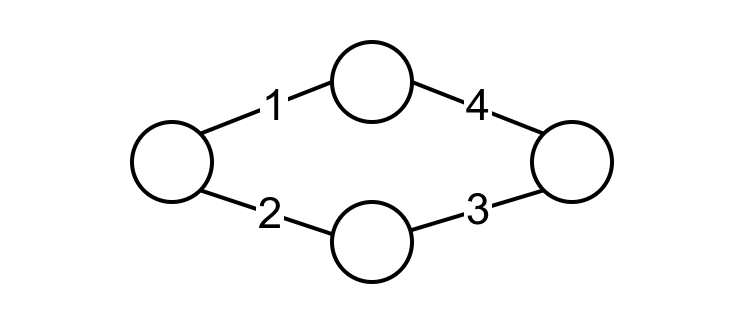
\includegraphics[width=0.6\textwidth]{graphics/graph_gewicht.png}
\end{minipage}
\hfill
\begin{minipage}{0.5\textwidth}
\subsubsection*{Knotengrad}
\begin{itemize}[leftmargin=*]
\item Anzahl Kanten die von einem Knoten ausgehen
\end{itemize}\
\\
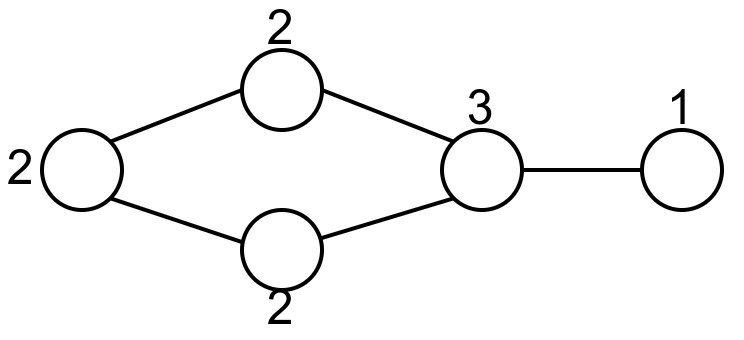
\includegraphics[width=0.6\textwidth]{graphics/graph_knotengrad.png}
\end{minipage}

\begin{minipage}{0.5\textwidth}
\subsubsection*{Euler-Zyklus/Eulersch}
\begin{itemize}[leftmargin=*]
\item Anfangszustand = Endzustand
\item Alle Knoten haben einen geraden Grad
\end{itemize}\
\\
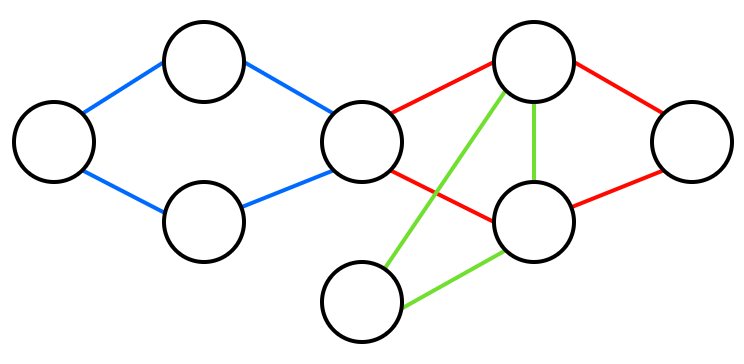
\includegraphics[width=0.6\textwidth]{graphics/graph_euler_zyklus.png}
\end{minipage}
\hfill
\begin{minipage}{0.5\textwidth}
\subsubsection*{Euler-Pfad}
\begin{itemize}[leftmargin=*]
\item Jede Kante wird genau einmal durchlaufen
\item Keine Kante wird mehrmals durchlaufen
\item Startknoten muss nicht gleich Endknoten sein
\item Genau zwei Knoten haben einen ungeraden Grad
\end{itemize}\
\\
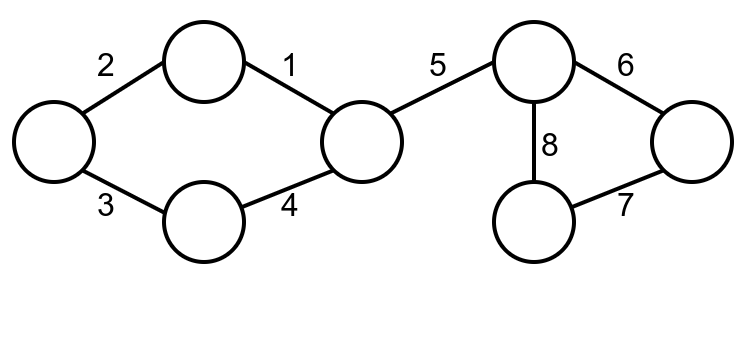
\includegraphics[width=0.6\textwidth]{graphics/graph_euler_pfad.png}\end{minipage}

\newpage

\begin{minipage}{0.5\textwidth}
\subsubsection*{Hamilton-Zyklus}
\begin{itemize}[leftmargin=*]
\item Anfangszustand = Endzustand
\item Alle Knoten geraden Grads
\end{itemize}\
\\
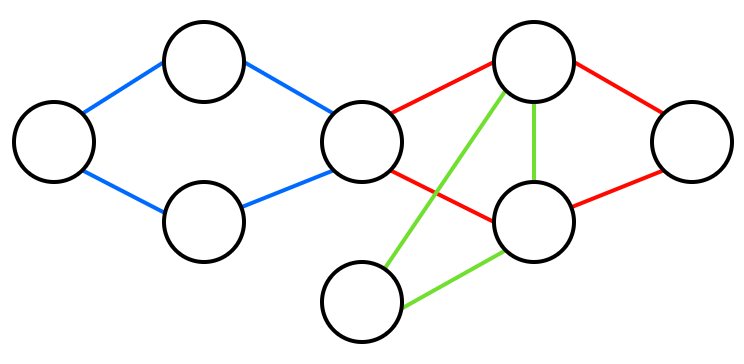
\includegraphics[width=0.6\textwidth]{graphics/graph_euler_zyklus.png}
\end{minipage}
\hfill
\begin{minipage}{0.5\textwidth}
\subsubsection*{Hamilton-Pfad}
\begin{itemize}[leftmargin=*]
\item Jede Kante wird genau einmal durchlaufen
\item Keine Kante wird mehrmals durchlaufen
\item Startknoten muss nicht gleich Endknoten sein
\end{itemize}\
\\
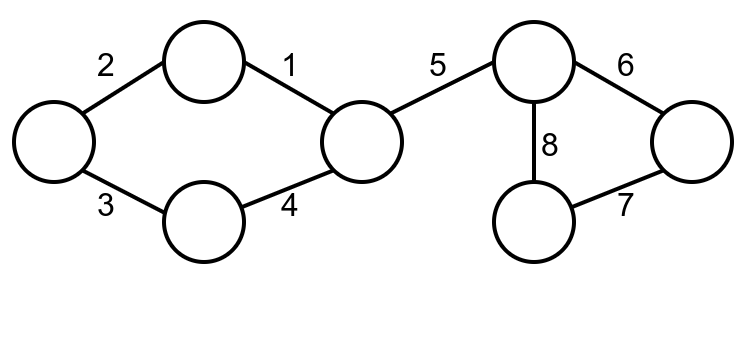
\includegraphics[width=0.6\textwidth]{graphics/graph_euler_pfad.png}\end{minipage}

\subsubsection*{Bipartit}

\begin{itemize}[leftmargin=*]
\item Man kann alle Knoten in zwei (disjunkte) Teilmengen/Gruppen aufteilen
\item Jede Verbindung geht dabei von einer Teilmenge/Gruppe in die andere
\item Es darf allerdings keine Verbindung der Knoten innerhalb der eigenen Teilmenge/Gruppe geben
\end{itemize}

\begin{figure}[h]
\centering
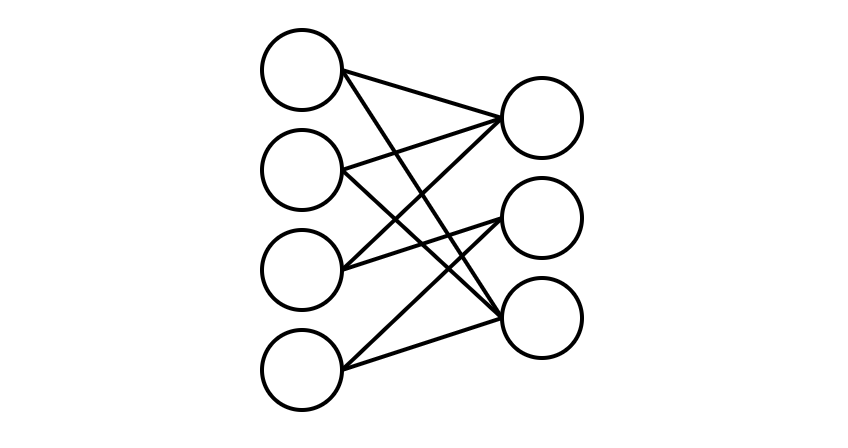
\includegraphics[width=0.4\textwidth]{graphics/graph_bipartit.png}
\end{figure}

\textbf{Beispiel:} Zeigen ob ein Graph bipartit ist

\begin{itemize}
\item Beliebigen Knoten auswählen und färben (z.B blau).
\item Alle benachbarte Knoten mit einer anderen Farbe färben (z.B grün)
\item Widerholen: Alle Knoten die an einen blauen Knoten angrenzen, grün und alle Knoten, die an einen grünen Knoten angrenzen, blau färben.
\item Prüfung: Wenn man auf einen Knoten stößt, der bereits gefärbt ist und dessen Farbe sich von der Farbe unterscheidet, die man ihm zuweisen möchten, dann ist der Graph \textit{nicht bipartit}. Wenn man alle Knoten ohne solche Konflikte färben konnte, ist der Graph \textit{bipartit}.
\item Die blauen Knoten sind am Ende die eine Teilmenge/Gruppe und die grünen Knoten sind am Ende die andere Teilmenge/Gruppe
\end{itemize}

\begin{figure}[h]
\centering
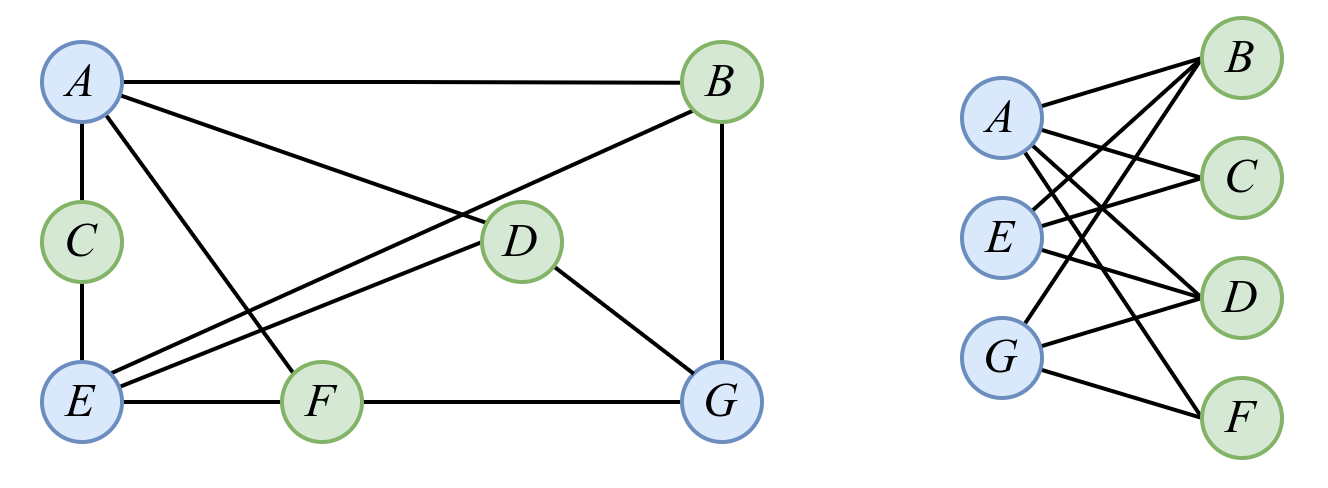
\includegraphics[width=0.75\textwidth]{graphics/graph_bipartit2.png}
\end{figure}

\newpage

\subsubsection*{Planar}

\begin{itemize}
\item Ein Graph ist planar, wenn man ihn so zeichnen kann, dass sich seine Kanten nirgendwo kreuzen.
\end{itemize}

\textbf{(Nicht) Planarität prüfen:}

\textbf{1 Methode:}

\begin{itemize}
\item $n = |V|$ (Anzahl Knoten) und $m = |E|$ (Anzahl Kanten) bestimmen
\item Hat der Graph einen Zyklus der Länge 3?
	\begin{itemize}
	\item[$\rightarrow$] \textbf{Ja:} $m \leq 3n - 6$
	\item[$\rightarrow$] \textbf{Nein:} $m \leq 2n - 4$
	\item Gilt $m \not \leq 3n - 6$ oder $m \not \leq 2n - 4$ ist der Graph \textit{nicht planar}
	\item \textbf{Achtung:} Die Formel macht nur eine Aussage darüber, ob der Graph nicht planar ist, aber nicht, ob ein Graph planar ist. Gilt also $m \leq 3n - 6$ oder $m \leq 2n - 4$ heißt es nicht, dass der Graph planar ist. Man kann also nur die Nichtplanarität überprüfen.
	\end{itemize}
\end{itemize}

\textbf{2 Methode:}

\begin{itemize}
\item Ist der 
\end{itemize}
